\documentclass[8pt]{article}
\usepackage{amsmath}
\usepackage{amssymb}
\usepackage{amsthm}
% \usepackage{amsfonts}
% \usepackage{amscd}
\usepackage{graphicx}
\usepackage{color}
\usepackage{hyperref}
\usepackage{enumerate}
% \usepackage{mathrsfs}
% \usepackage{tikz}
% \usepackage{tikz-cd}
\usepackage{listings}
\usepackage{xcolor}
\usepackage{textcomp}
\usepackage{xcolor}
\usepackage{verbatim}
<<<<<<< HEAD
\usepackage{subfig}
=======
\usepackage{url}
\usepackage{fancyhdr}
\usepackage{blindtext}
\usepackage{multicol}

% Columns
\setlength{\columnsep}{-1cm}
>>>>>>> 60afbbe36b36476e012367c20bd58e7d8a5fa704

% To define colors
\definecolor{commentgreen}{RGB}{40, 180, 20}
% \definecolor{commentgreen}{RGB}{2,112,10}
\definecolor{eminence}{RGB}{108,48,130}
\definecolor{weborange}{RGB}{160,1,130}
\definecolor{frenchplum}{RGB}{30, 30, 210}

% To EXTREMELY customiza the style of the listings package
\lstset{
    basicstyle=\ttfamily,
    columns=fullflexible,
    breaklines=true,
    breakatwhitespace=true,
    frame=single,
    framerule=0.1pt,
    framesep=5mm,
    showstringspaces=false,
    showspaces=false,
    showtabs=false,
    tabsize=4,
    % numbers=left,
    numberstyle=\tiny,
    numbersep=5pt,
    stepnumber=1,
    numberblanklines=true,
    captionpos=b,
    backgroundcolor=\color{gray!10},
    keywordstyle=\color{weborange}, %\bfseries\underbar
    commentstyle=\color{commentgreen},
    stringstyle=\color{red},
    % identifierstyle=\color{pink},
    emph={as, from}, emphstyle=\color{weborange},
    % emph={[2]import}, emphstyle={[2]\color{blue}},
    breakautoindent=true,
    breakindent=2em,
    keepspaces=true,
    morekeywords={for, while, if, else, elif, def, return, print, in, range, len, enumerate, zip, list, tuple, set, dict, True, False, None, and, or, not, is, in, not in, from, import, as, try, except, finally, raise, assert, pass, del, global, nonlocal, lambda, with, yield, class, break, continue, async, await},
    xleftmargin=1.5cm,
    xrightmargin=1.5cm,
    frameround=tttt,
    rulecolor=\color{gray!40},
    % To make bigger the radius of the frame:
    frameround=2mm,
    }
    
    % To EXTREMELY customiza the style of the verbatim inline
    \newcommand{\code}[1]{\texttt{\color{frenchplum}{#1}}}
    
    % Margins = 2cm and 4cm
    \usepackage[margin=2cm, left=4cm, right=4cm]{geometry}
    
    % Fonts and language in Spanish
    \usepackage[spanish]{babel}
    \usepackage[utf8]{inputenc}
    
    % Fancy
    \pagenumbering{arabic}
    \pagestyle{fancy}
    \lfoot{\small\textit{Jorge Antonio Gómez García}}
    \rfoot{\small\textit{Saud Antonio Morales González}}
    % To use fancyhdr margins
    \renewcommand{\headrulewidth}{0.4pt}

    % Rename things
    \renewcommand{\contentsname}{Contenido}
    \renewcommand{\sectionautorefname}{Sección}
    \renewcommand{\subsectionautorefname}{Subsección}
    \renewcommand{\subsubsectionautorefname}{Subsubsección}
    \renewcommand{\figureautorefname}{Figura}
    \renewcommand{\tableautorefname}{Tabla}
    \renewcommand{\equationautorefname}{Ecuación}
    \renewcommand{\appendixautorefname}{Apéndice}
    \renewcommand{\appendixname}{Apéndices}

\title{Teoremas del límite: la ley de los grandes números y el teorema límite central}
\author{Jorge Antonio Gómez García \\ Saud Antonio Morales González}
\date{\today}


% ##################################################################


\begin{document}
\maketitle

\begin{multicols}{2}
    \begin{abstract}
        En este trabajo se presenta una breve explicación de la ley de los grandes números y del teorema del límite central, así como su aplicación en el ámbito de la probabilidad y la estadística. Los autores presentan ejemplos de aplicación de estos teoremas en el lenguaje de programación Python a la vez que se explican los conceptos teóricos que se utilizan para desarrollar y entender los ejemplos. Los tres temas centrales son: La ley débil de los grandes números, la ley fuerte de los grandes números y el teorema del límite central. Cada ejemplo incluye el lema del teorema así como una referencia a la demostración del mismo.
    \end{abstract}

\end{multicols}

\paragraph*{\rule{\textwidth}{0.4pt}}

\tableofcontents
\vspace*{1cm}
\paragraph*{\rule{\textwidth}{0.4pt}}


% ##################################################################


\section*{Introducción}
\addcontentsline{toc}{section}{Introducción}

La ley de los grandes números y el teorema límite central son dos teoremas que se encuentran en el ámbito de la probabilidad y la estadística. Estos teoremas son de gran importancia en la teoría de la probabilidad, ya que son los que permiten establecer la convergencia de las variables aleatorias; en el caso del teorema límite central la convergencia se da a una distribución normal. Lo que permite realizar inferencias estadísticas sobre la población a partir de una muestra. En el presente trabajo, los autores se enfocarán en la explicación breve de estos teoremas, así como en la aplicación de los mismos en el ámbito de la estadística con el lenguaje de programación Python. Infiriendo convergencias con cada uno de ellos.

\pagebreak


% ##################################################################

\section{La ley de los grandes números}

\begin{quote}
    \textit{En la teoría de la probabilidad, bajo el término genérico de ley de los grandes números se engloban varios teoremas que describen el comportamiento del promedio de una sucesión de variables aleatorias conforme aumenta su número de ensayos. \vspace*{0.15cm} \\ Estos teoremas prescriben condiciones suficientes para garantizar que dicho promedio converja [...] al promedio de las esperanzas de las variables aleatorias involucradas. Las distintas formulaciones de la ley de los grandes números (y sus condiciones asociadas) especifican la convergencia de formas distintas.}\footnote{Colaboradores de los proyectos Wikimedia, "Ley de los grandes números", Wikipedia, la enciclopedia libre, 28 de enero de 2006.}
\end{quote}

La ley de los grandes números se divide en dos teoremas: la ley débil de los grandes números y la ley fuerte de los grandes números. La ley débil de los grandes números se refiere a la convergencia en probabilidad de la secuencia de las medias muestrales, mientras que la ley fuerte de los grandes números se refiere a la convergencia \textit{casi segura} de la secuencia de las medias muestrales.

% ##################################################################

\subsection{Ley débil de los grandes números}

\begin{quote}
    \textbf{\textit{--- La secuencia de las medias muestrales converge en probabilidad a la media poblacional.}}
\end{quote}

Sea $\{X_n\}$ una secuencia de variables aleatorias independientes tales que $\text{E}[X_n] = \mu$ y $\text{var}(X_n) \leq M$ para cada $n \geq 1$. Entonces, la siguiente secuencia de variables aleatorias converge a $\mu$ en probabilidad:

\begin{align*}
    \overline{X}_n &:= \frac{1}{n}(X_1 + \cdots + X_n) = \frac{1}{n}\sum_{i=1}^n X_i \longrightarrow \mu \quad \text{en probabilidad}.
\end{align*}

De esta ecuación tenemos que:

\begin{align*}
    \text{E}[\overline{X}^2_n] &\rightarrow \mu^2 \\
\end{align*}

% Texto centrado con el texto "leyenda":

\fbox{\textbf{Ejemplo de la ley débil de los grande números:}} \\\\

Considere el siguiente ejemplo: Sean $X_1, X_2, \ldots$ variables aleatorias independientes con distribución exponencial, tal que $X_i \sim \text{Exp}(\lambda)$. El segundo momento $\text{E}[\overline{X}^2_i]$ de $X_i$, con $m$ diferentes valores de $\omega$, puede ser simulado en Python de la siguiente manera:

\vspace*{0.3cm}

Importamos las librerías necesarias y definimos los parámetros:

\begin{lstlisting}[language=Python]
# Librerias
import numpy as np
import matplotlib.pyplot as plt

# Parametros
media_exp = 2   # beta = 0.5
n = 10000       # Numero de variables aleatorias
m = 500         # Numero de experimentos
\end{lstlisting}

Generamos $m$ muestras de $n$ variables aleatorias con distribucion exponencial:

\begin{lstlisting}[language=Python]
x = np.random.exponential(media_exp, (m,n))
    # (m,n) es una matriz (filas, columnas)
\end{lstlisting}

Obtenemos la media de cada una de las muestras:

\begin{lstlisting}[language=Python]
x_barra = np.mean(x, axis=1)
    # axis=1: calcula la media de cada fila
    # (m, 1) es un vector columna
\end{lstlisting}

Obtenemos el segundo momento de cada una de las muestras:

\begin{lstlisting}[language=Python]
segundo_momento_x_barra = np.mean(x_barra**2)

print(segundo_momento_x_barra)
    # Resultado: 3.9989201200495708
\end{lstlisting}

Como puede ver, el segundo momento está muy aproximado al segundo momento real de la distribución exponencial, que es $\text{E}[\overline{X}^2_i] = 1/\beta^2 = 4$. Así, usando la definición de varianza, podemos observar que la varianza de la media de las muestras tiende a cero:

\begin{align*}
    \text{var}(\overline{X}_n) &\longrightarrow 0
\end{align*}

Recordando que la varianza es el segundo momento menos el cuadrado del primer momento, tenemos:

\begin{lstlisting}[language=Python]
varianza_x_barra = segundo_momento_x_barra - np.mean(x_barra)**2

print(varianza_x_barra)
    # Resultado: 0.00015
\end{lstlisting}

\vspace*{0.3cm}

¿Qué describe el código anterior? Primero, determinamos los parámetros de la distribución exponencial. En este caso la media está definida como \code{media\_exp = 2}. A su vez, establecimos una cantidad de variables aleatorias \code{n = 10000} y un número de experimentos \code{m = 500}. Luego, generamos $m$ muestras de $n$ variables aleatorias con distribución exponencial. A continuación, calculamos la media de cada una de las muestras. Finalmente, calculamos el segundo momento de cada una de las muestras. Como puede ver, el segundo momento está muy aproximado al segundo momento real de la distribución exponencial, que es $\text{E}[\overline{X}^2_i] = 1/\beta^2$. De esta manera, hemos comprobado que la ley débil de los grandes números se cumple para la distribución exponencial.\\

Por último, si el lector gusta ver la demostración de la ley débil de los grandes números, puede consultar el siguiente enlace: \url{https://www.mat.uc.cl/~aramirez/pcap2.pdf}.


% ##################################################################

\subsection{Ley fuerte de los grandes números}



% ##################################################################

\section{El teorema límite central}

Sean $X_1, X_2, ..., X_n$ n variables aleatorias IID con una distribucion de probabilidad no específicada y que tienen una media $\mu$ y una varianza $\sigma^2$ finita. El promedio muestral $\overline{X} = (X_1, X_2, ..., X_n)/n$ tiene una distribución con media $\mu$ y varianza $\sigma^2/n$ que tiende hacia una distribución normal conforme $n$ tiende a $\infty$. En otras palabras, la variable aleatoria $(\overline{X}-\mu)/(\sigma/\sqrt{n})$ tiene como limite una distribución normal estándar.\footnote{George C. Canavos, \textit{Probabilidad y estadística: aplicaciones y métodos}, trad. Edmundo Urbina (Ciudad de México: McGraw Hill, 1988), 230.} 

La demostración de este teorema puede ser consultada en las páginas 247-249 del libro de \textit{Probabilidad y estadística: aplicaciones y métodos} de George Canavos.

\subsection{Teorema de Moivre-Laplace}

Sea $X$ una variable aleatoria binomial con media $np$ y desviación estandar $\sqrt{np(1-p)}$. La distribución de la variable aleatoria tiende a la normal estandar conforme el número de ensayos independientes $n \rightarrow \infty$. \footnote{Canavos, \textit{Probabilidad y estadística: aplicaciones y métodos}, 141-142.} En otras palabras, una distribución binomial tenderá a la normal estándar conforme el número de ensayos vaya aumentando.

\
Para ilustrarlo se graficaran las funciones de masa de probabilidad de que una moneda caiga cara en $n$ experimentos. Donde $n$ tomará valores cada vez más grandes.\

\begin{figure}
        \subfloat[n=5]{
            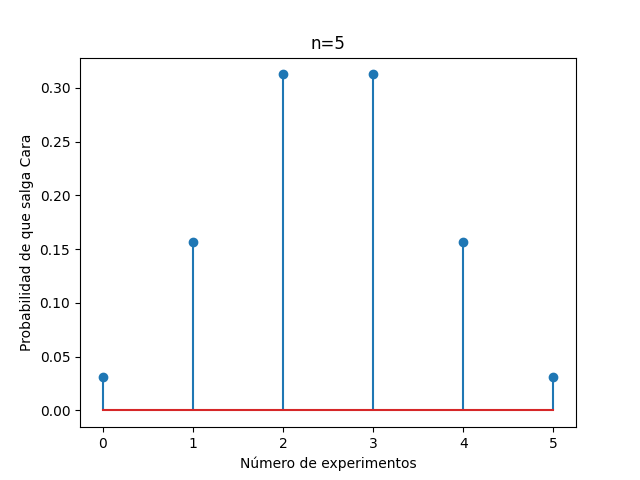
\includegraphics[scale=.4]{n=5.png}}
        \subfloat[n=10]{
            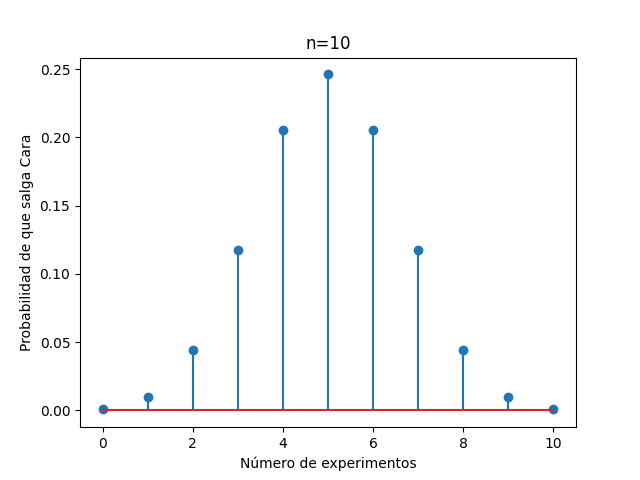
\includegraphics[scale=.4]{n=10.png}}\\
        \subfloat[n=30]{
            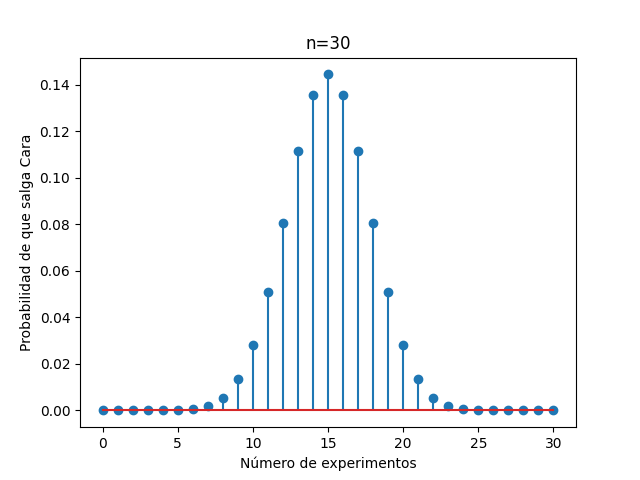
\includegraphics[scale=.4]{n=30.png}}
        \subfloat[n=50]{
            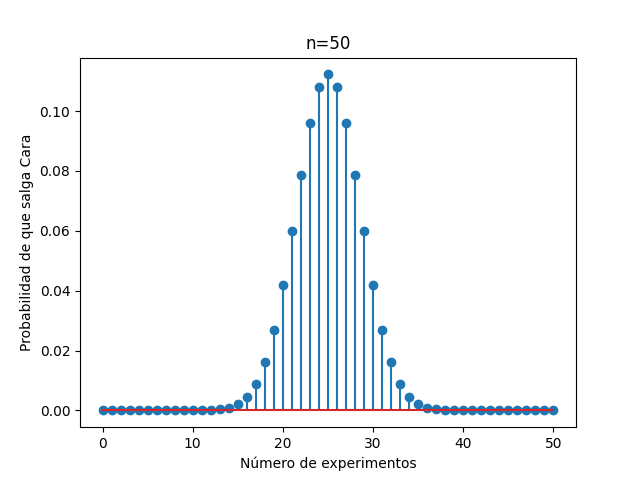
\includegraphics[scale=.4]{n=50.png}}\\
        \subfloat[n=100]{
            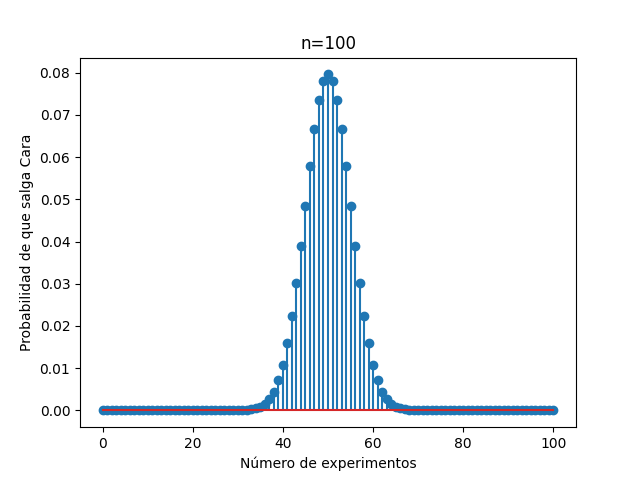
\includegraphics[scale=.4]{n=100.png}}
        \subfloat[n=500]{
            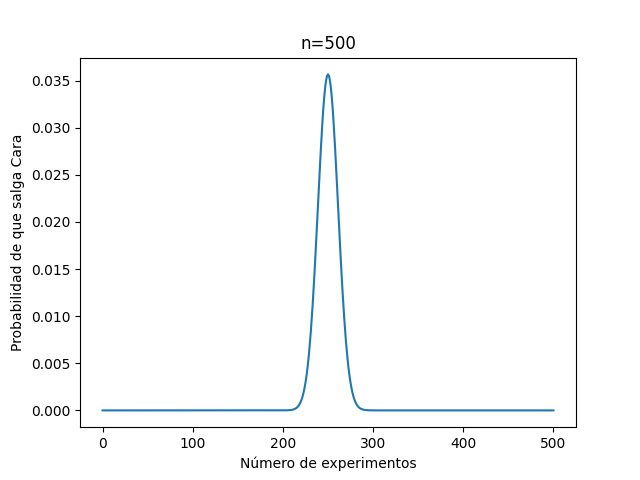
\includegraphics[scale=.4]{n=500.png}}
        \caption{Teorema de Moivre-Laplace}
        \label{f:animales}

\end{figure}

\
Como es observado, mientras más aumenta la cantidad de experimentos realizados, más se asemeja la función de masa de probabilidad de la distribución binomial a la función de densidad de probabilidad de la distribución normal.


% ##################################################################

\section{Conclusiones}


\end{document}